\section{Auswertung}
\label{sec:Auswertung}

\DeclareSIUnit{\rad}{rad} %Damit "rad" in \SI verwendet werden kann

\subsection{Messung der Zeitkonstanten $RC$ über die Entladekurve}
Die in Aufgabenteil a) verwendete Frequenz beträgt $\SI{420}{\hertz}$. Aus dem Zusammenhang für den Entladevorgang eines Kondenators folgt
\begin{align}
    \symup{ln}(\frac{U}{U_{0}}) = -\frac{1}{RC}\cdot t.
\end{align}
Mithilfe von numpy \cite{numpy} und matplotlib \cite{matplotlib} werden die Messwerte, die
\autoref{tab:wertea} zu entnehmen sind, halblogarithmisch in \autoref{fig:plot_a} geplottet und es wird eine Regressionsgerade erstellt.

\begin{table}[H]
    \centering
    \caption{Messwerte zu Aufgabe a).}
    \label{tab:wertea}
    \begin{tabular}{c c}
        \toprule
        $U \:/\:$ V & $t \:/\:$ ms \\
        \midrule
        0,55 & 0,00 \\
        0,50 & 0,02 \\
        0,44 & 0,04 \\
        0,40 & 0,05 \\
        0,36 & 0,06 \\
        0,32 & 0,08 \\
        0,26 & 0,10 \\
        0,24 & 0,12 \\
        0,18 & 0,14 \\
        0,12 & 0,16 \\
        0,1 & 0,18 \\
        0,04 & 0,20 \\
        0,00 & 0,22 \\
        -0,04 & 0,24 \\
        -0,06 & 0,26 \\
        -0,10 & 0,28 \\
        -0,14 & 0,30 \\
        -0,16 & 0,32 \\
        -0,18 & 0,34 \\
        -0,22 & 0,36 \\
        -0,24 & 0,38 \\
        -0,28 & 0,40 \\
        -0,30 & 0,42 \\
        -0,32 & 0,44 \\
        -0,34 & 0,46 \\
        -0,38 & 0,48 \\
        -0,40 & 0,5 \\
        -0,42 & 0,52 \\
        -0,44 & 0,54 \\
        -0,46 & 0,56 \\
        -0,48 & 0,58 \\
        -0,50 & 0,6 \\
        \bottomrule
    \end{tabular}
\end{table}

\begin{figure}[H]
    \centering
    \includegraphics{build/plota.pdf}
    \caption{Halblogarithmischer Plot zu Aufgabenteil a) mit Ausgleichsgerade.}
    \label{fig:plot_a}
  \end{figure}

Die Parameter der Ausgleichsgeraden vom Typ $\symup{ln}(\frac{U}{U_{0}}) = m \cdot t + b$ werden zu den folgenden Werten ermittelt
\begin{align*}
    m = \SI{-0.697 (0.014)}{\per\milli\second}, \\
    b = 1.087 \.\pm 0.014. \\
\end{align*}
Dadrch ergibt sich eine Zeitkonstante $RC$ von 
\begin{align*}
    RC = \SI{0.705 (0.014)}{\per\second}.
\end{align*}



\subsection{Bestimmen der Zeitkonstanten $RC$ über die Frequenzabhängigkeit der Amplitude}
Aus \autoref{tab:wertebc} sind die Messwerte zu Aufgabenteil b) und c) zu entnehmen.
\begin{table}[H]
    \centering
    \caption{Messwerte zu Aufgabe b) und c).}
    \label{tab:wertebc}
    \begin{tabular}{c c c c c}
        \toprule
        $f \:/\:\si{\kilo\hertz}$ & $A_1 \:/\: \si{\volt}$ & $A_1 \:/\: \si{\volt}$ & $a \:/\: \si{\milli\second}$ & $b \:/\: \si{\milli\second}$ \\
        \midrule
        3,085 & 4,2 & 0,1100 & 0,0300 & 0,1800 \\
        6 & 4,2 & 0,0600 & 0,0240 & 0,0680 \\
        9 & 4,2 & 0,0480 & 0,0180 & 0,070 \\
        12 & 4,2 & 0,0360 & 0,0120 & 0,0460 \\
        15 & 4,2 & 0,0260 & 0,0100 & 0,0380 \\
        18 & 4,2 & 0,0220 & 0,0100 & 0,0240 \\
        21 & 4,2 & 0,0180 & 0,0080 & 0,0260 \\
        24 & 4,2 & 0,0150 & 0,0070 & 0,0230 \\
        27 & 4,2 & 0,0130 & 0,0060 & 0,0210 \\
        30 & 4,2 & 0,0110 & 0,0050 & 0,0190 \\
        33 & 4,2 & 0,0100 & 0,0050 & 0,0165 \\
        36 & 4,2 & 0,0085 & 0,0050 & 0,0150 \\
        39 & 4,2 & 0,0075 & 0,0045 & 0,0114 \\
        42 & 4,2 & 0,0070 & 0,0040 & 0,0135 \\
        45 & 4,2 & 0,0060 & 0,0040 & 0,0120 \\
        48 & 4,2 & 0,0060 & 0,0035 & 0,0115 \\
        51 & 4,2 & 0,0050 & 0,0030 & 0,0110 \\
        54 & 4,2 & 0,0050 & 0,0030 & 0,0100 \\
        57 & 4,2 & 0,0045 & 0,0030 & 0,0100 \\
        60 & 4,2 & 0,0040 & 0,0025 & 0,0095 \\
        \bottomrule
    \end{tabular}
\end{table}


\begin{figure}[H]
    \centering
    \includegraphics[width=0.75\textwidth]{build/plotb.pdf}
    \caption{Frequenzabhängiges Amplitudenverhältnis.}
    \label{fig:Plotb}
\end{figure}
Aus (\ref{eqn:Amplitude}) ergibt sich ein Zusammenhang für die Ausgleichsrechnung der Zeitkonstanten $RC$
\begin{align}
    \frac{A(\omega)}{U_0} = \frac{1}{\sqrt{1+\omega^2R^2C^2}}.
    \label{eqn:ausgl}
\end{align}
Aus \autoref{fig:Plotb} ist die graphische Abbildung der Messwerte aus \autoref{tab:wertebc} zu entnehmen, wodurch mithilfe der Python
Erweiterungen matplotlib \cite{matplotlib}, numpy \cite{numpy} und scipy \cite{scipy} die Zeitkonstanten $RC$ bestimmt wird.
Es folgt eine Zeitkonstante von
\begin{align*}
    RC = \SI{1.88 (1.55)}{\per\second}.
\end{align*}

\subsection{Phasenverschiebung des RC-Kreises}
Ein Zusammenhang zwischen der Phasenverschiebung von $U_{\text{C}}$ und $U_0$ und der Frequenz der Spannungsquelle wird durch
die folgende Gleichung beschrieben
\begin{align}
    \varphi(\omega) = -\arctan{-\omega\cdot RC}.
    \label{eqn:phasev}
\end{align}
Dabei wird die Phase über $\varphi = 2\pi\frac ab$ bestimmt. Die Messwerte sind \autoref{tab:wertebc} zu entnehmen.
Das Wertepaar $\{f\,[\si{\hertz}], \varphi(\omega)\, [\si{\rad}]\}$ wird in \autoref{fig:plotc} dargestellt.
\begin{figure}[H]
    \centering
    \includegraphics[width=0.75\textwidth]{build/plotc.pdf}
    \caption{Graphische Darstellung der Phasenverschiebung.}
    \label{fig:plotc}
\end{figure}
Es ist jedoch nicht möglich aus den gemessenen Werten eine Zeitkonstante $RC$ zu bestimmen, worauf näher in \autoref{sec:Diskussion}
eingegangen wird.

Die Werte werden zusätzlich in einem Polarplot in \autoref{fig:plotd} visualisiert, aus dem sich aus denselben Gründen 
keine Informationen entnehmen lassen.
\begin{figure}[H]
    \centering
    \includegraphics[width=0.75\textwidth]{build/plotd.pdf}
    \caption{Polarplot zu der Phasenverschiebung $\varphi$.}
    \label{fig:plotd}
\end{figure}

\subsection{RC-Kreis als Integrator}
\label{subsec:integr}
Aus \autoref{subsec:int} folgt, dass ein RC-Kreis auch als Integrator dienen kann.
Für eine Rechteckspannung mit konstanten Spannungsabschnitten ist eine Stammfunktion mit einem linearen Spannungsbild zu erwarten.
In \autoref{fig:d.3} ist ebendies dargestellt.
Bei einer angelegten Dreiecksspannung mit linearem Verlauf ist ein quadratischer Spannungsverlauf zu erwarten.
Durch den zeitlichen Verlauf ergibt sich somit eine sinusförmiger Spannungsverlauf, wie er in \autoref{fig:d.2} dargestellt ist.
Durch Integration einer Sinusspannung der Form 
\begin{align*}
    f(\omega) = \sin{\omega t},
\end{align*}
ist eine Cosinunsspannung der Form
\begin{align*}
    f(\omega) = \frac{1}{\omega} \cos{\omega t}
\end{align*}
zu erwarten, was in \autoref{fig:d.1} abgebildet wird.
\begin{figure}[H]
    \centering
    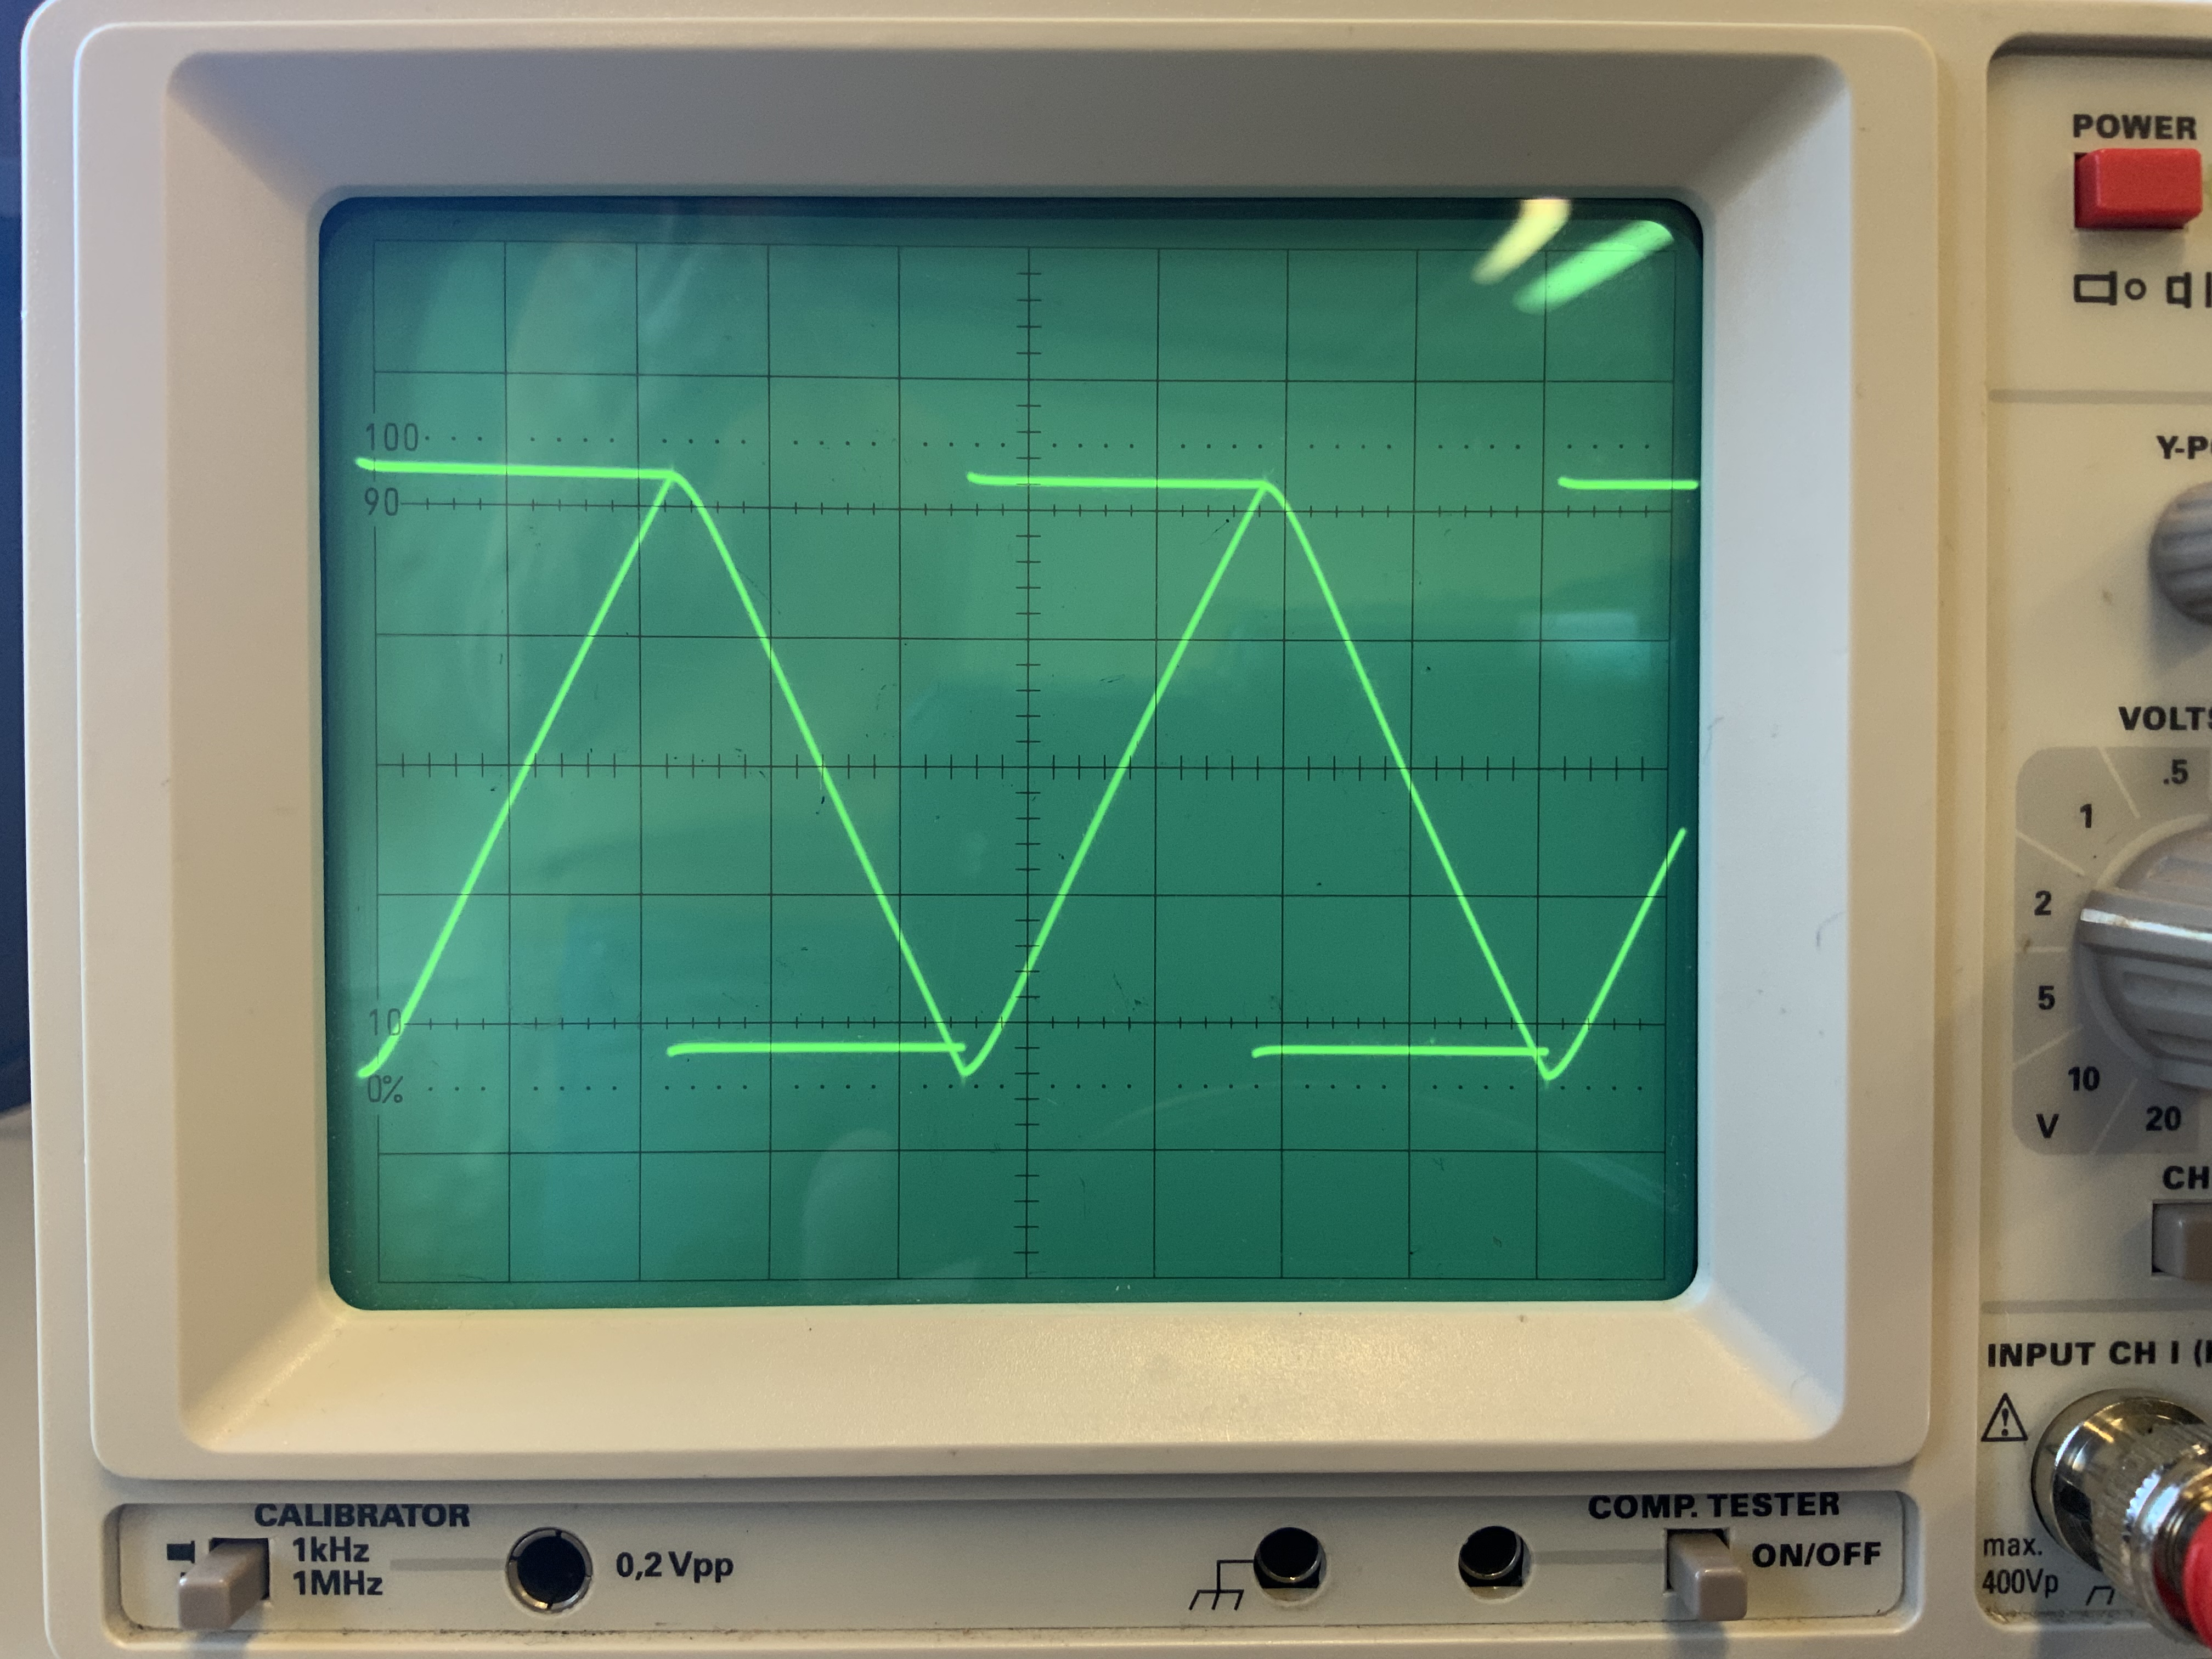
\includegraphics[width=0.75\textwidth]{Dateien/d.3.jpeg}
    \caption{Angelegte Rechteckspannung am RC-Kreis.}
    \label{fig:d.3}
\end{figure}
\begin{figure}[H]
    \centering
    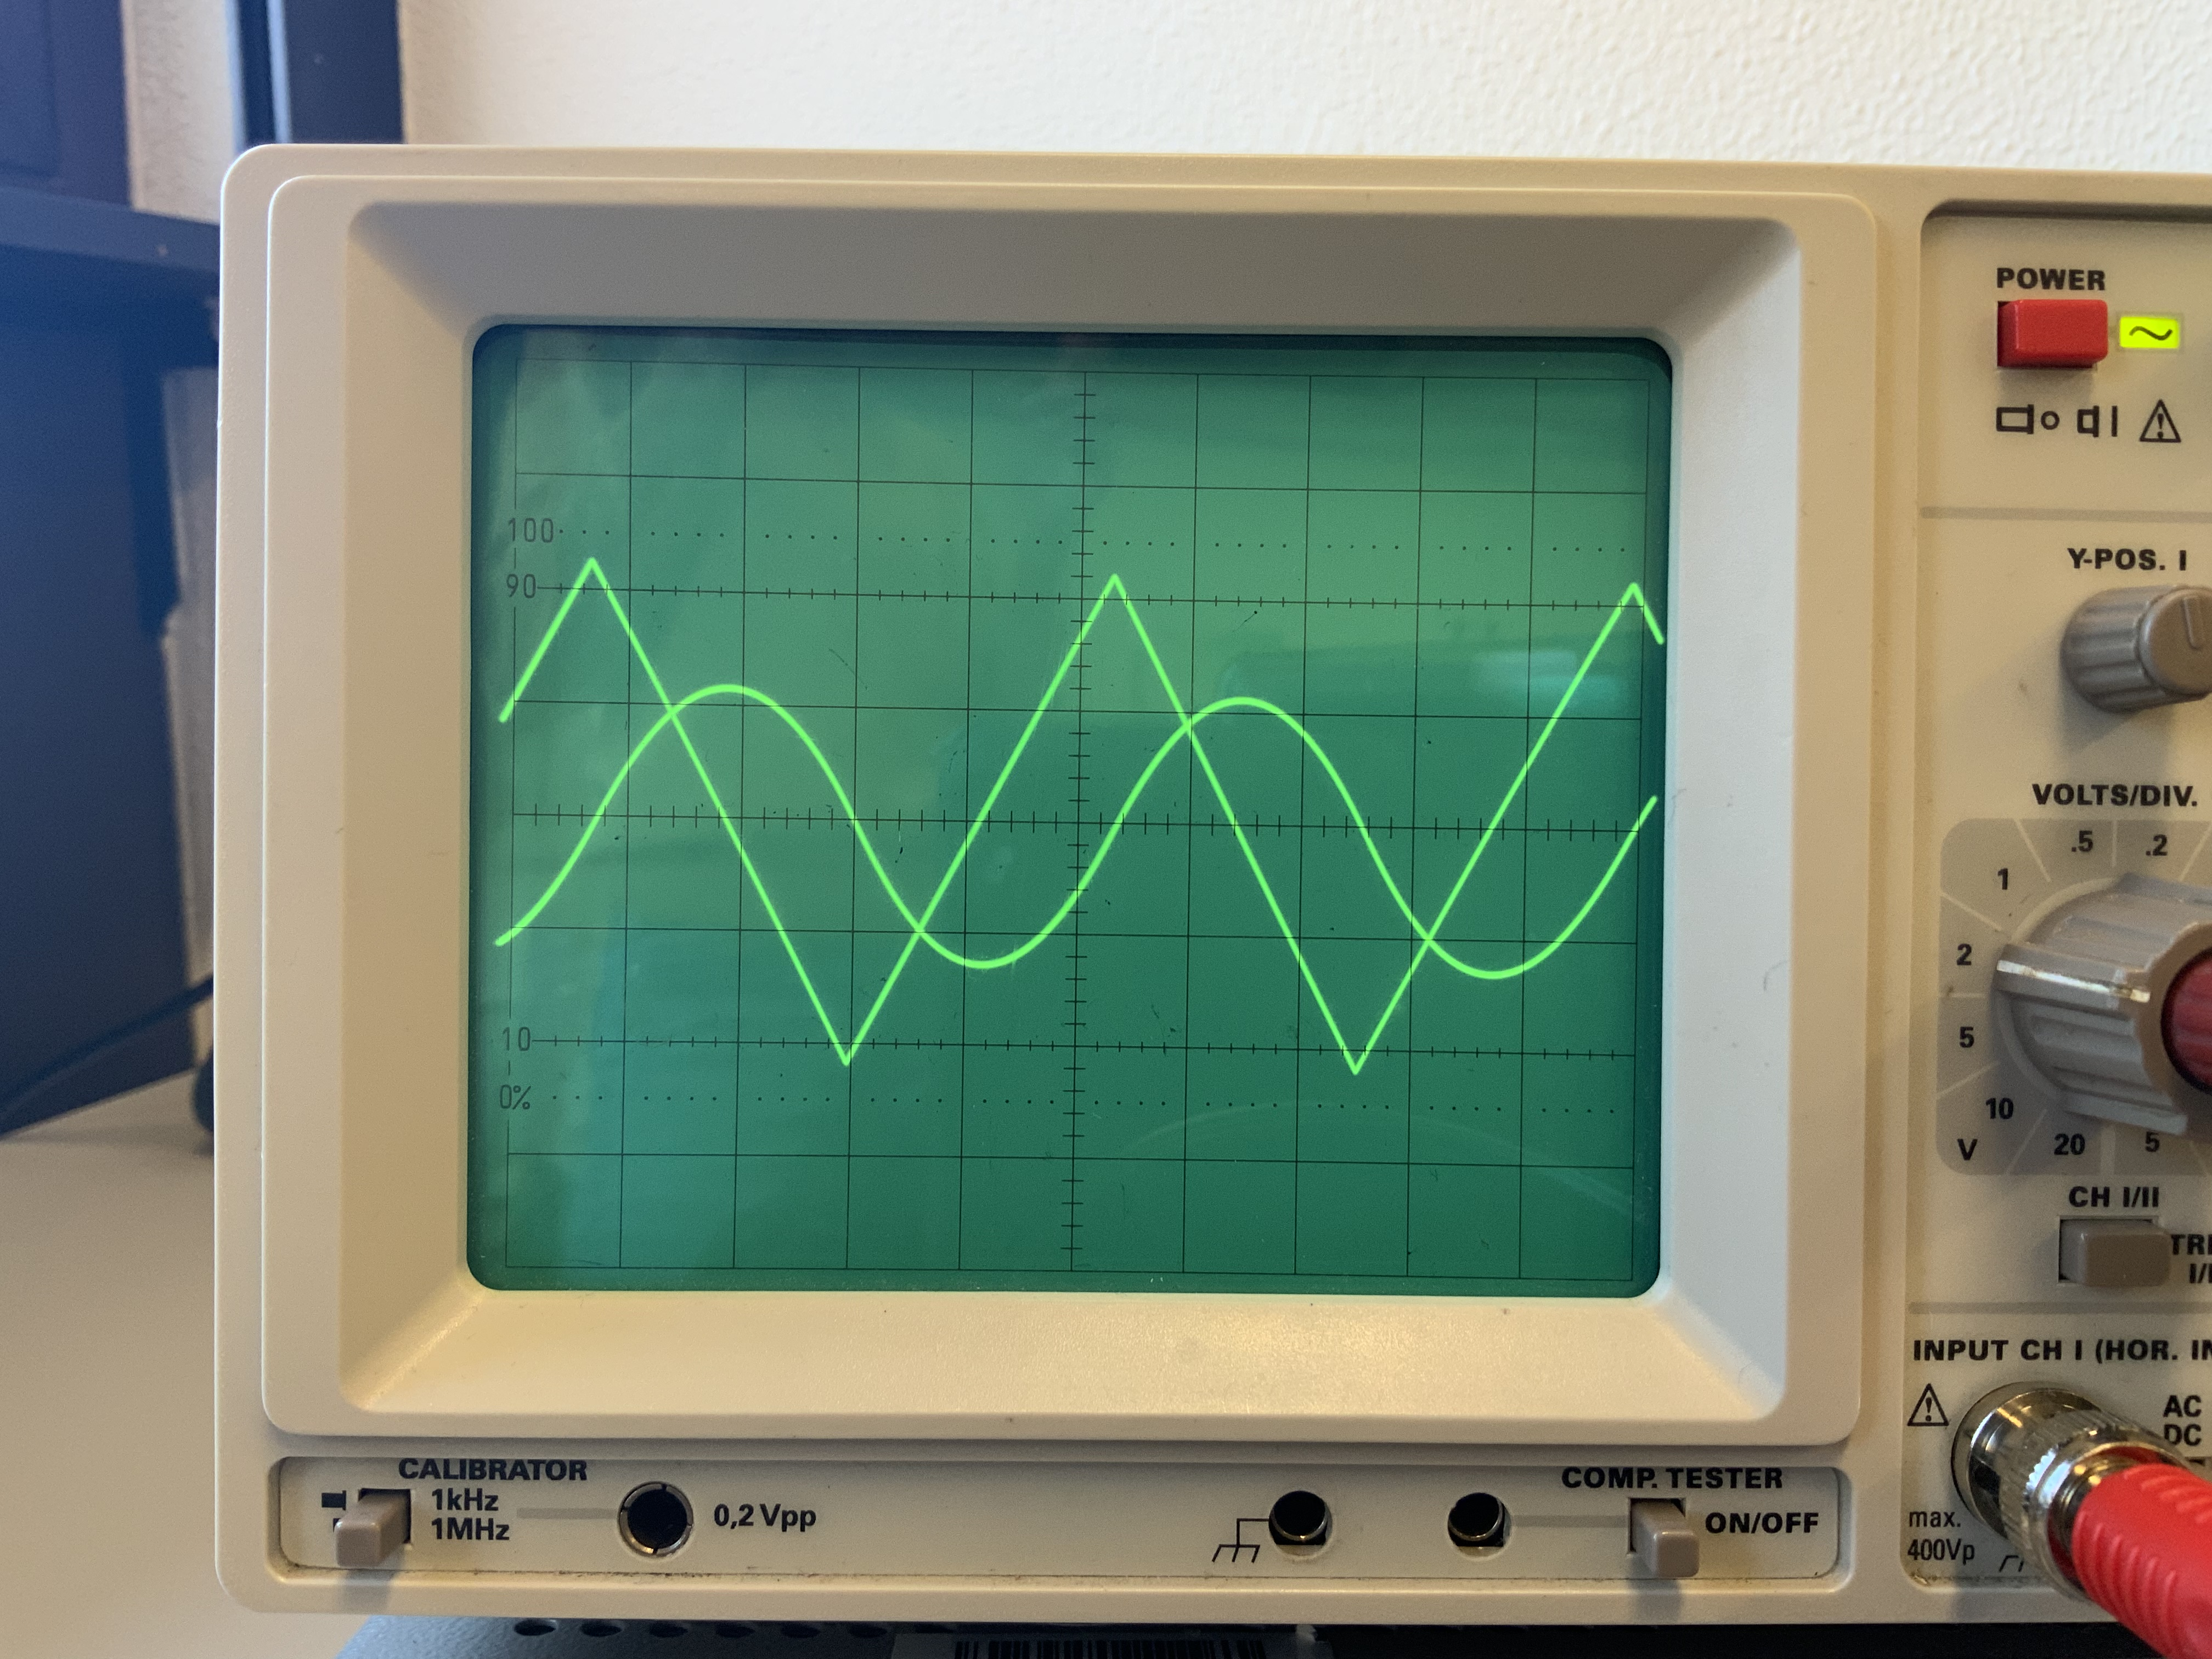
\includegraphics[width=0.75\textwidth]{Dateien/d.2.jpeg}
    \caption{Angelegte Dreiecksspannung am RC-Kreis.}
    \label{fig:d.2}
\end{figure}
\begin{figure}[H]
    \centering
    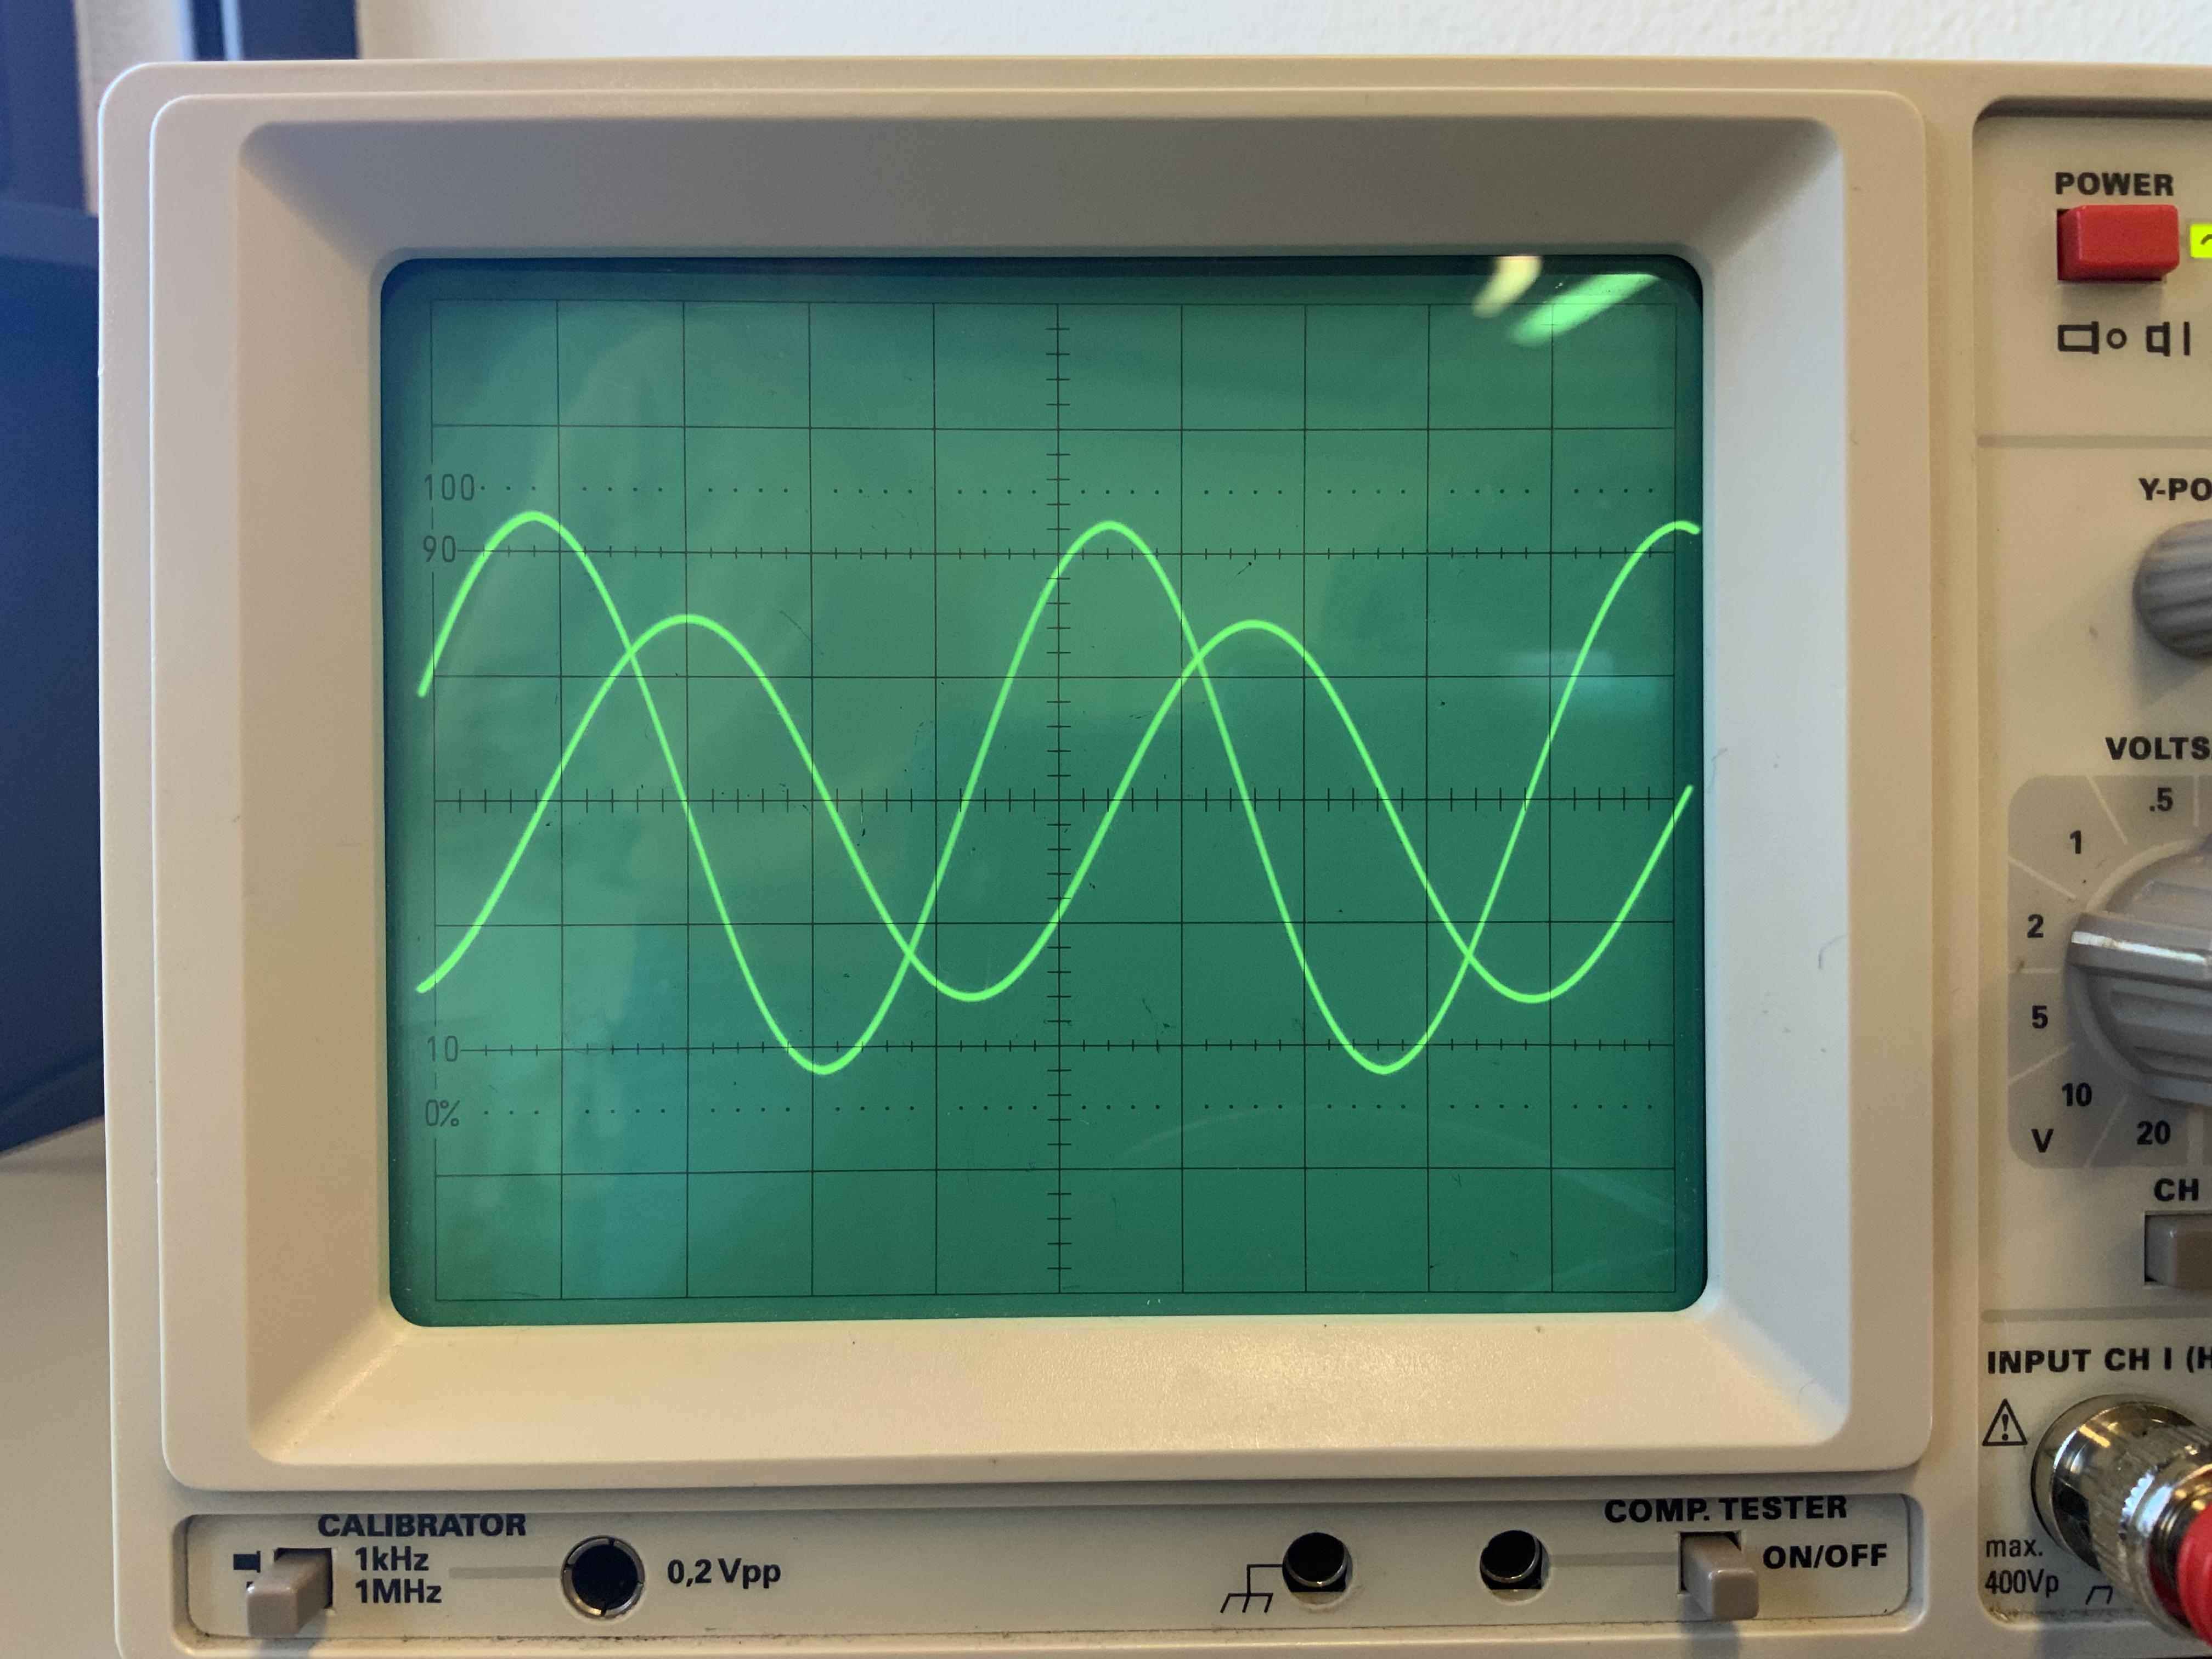
\includegraphics[width=0.75\textwidth]{Dateien/d.1.jpeg}
    \caption{Angelegte Sinusspannung am RC-Kreis.}
    \label{fig:d.1}
\end{figure}